\documentclass[11pt,a4paper]{article}
\usepackage[utf8]{inputenc}
\usepackage[T1]{fontenc}
\usepackage{amsmath,amssymb}
\usepackage{booktabs}
\usepackage{graphicx}
\usepackage{hyperref}
\usepackage{listings}
\usepackage{xcolor}
\usepackage[margin=1in]{geometry}
\usepackage{caption}
\usepackage{subcaption}
\usepackage{enumitem}
\usepackage{authblk}
\usepackage{multicol}
\usepackage{float}

\definecolor{codegreen}{rgb}{0,0.6,0}
\definecolor{codegray}{rgb}{0.5,0.5,0.5}
\definecolor{codepurple}{rgb}{0.58,0,0.82}
\definecolor{backcolour}{rgb}{0.95,0.95,0.95}

\lstdefinestyle{mystyle}{
    backgroundcolor=\color{backcolour},
    commentstyle=\color{codegreen},
    keywordstyle=\color{codepurple},
    numberstyle=\tiny\color{codegray},
    stringstyle=\color{codegreen},
    basicstyle=\ttfamily\small,
    breakatwhitespace=false,
    breaklines=true,
    captionpos=b,
    keepspaces=true,
    numbers=left,
    numbersep=5pt,
    showspaces=false,
    showstringspaces=false,
    showtabs=false,
    tabsize=2,
    frame=single
}
\lstset{style=mystyle}

\title{JIT LoRA: Real-Time Conversational Knowledge Injection\\on Apple Silicon via MLX}

\author[1]{E. Elbaz}
\affil[1]{Independent Research}

\date{March 2026}

\begin{document}

\maketitle

\begin{abstract}
We present a system for just-in-time (JIT) LoRA training that modifies a running language model's weights mid-conversation on consumer Apple Silicon hardware. Using MLX-native autograd~\cite{mlx2023} for gradient-based LoRA~\cite{hu2021lora} adaptation, the system---J.A.R.V.I.S., a voice-enabled AI assistant---updates its own weights after every response via background backpropagation. We validate on three evaluation tracks: (1)~a controlled fictional-fact experiment achieving 4/4 recall ($n=4$), (2)~a cross-domain scaling test with 41 interlocked facts achieving 69\% direct recall with 50\% multi-hop reasoning, and (3)~a statistically rigorous evaluation against \textbf{35 real-world facts} the model verifiably did not know, yielding \textbf{58.1\% recall} (95\% Wilson CI: [48.5\%, 67.1\%], $n=105$ pooled across 3 independent trials) with \textbf{100\% general knowledge preservation} (CI: [94.0\%, 100.0\%], $n=60$). Training completes in 70 seconds for 35 facts on a 2B-parameter model. Per-category analysis reveals strong performance on structurally distinctive facts (Sports 88.9\%, Awards 85.7\%, Weather 80.0\%) with systematic failure on structurally homogeneous facts (Deaths 18.2\%), establishing both the capabilities and limits of JIT LoRA on small models.
\end{abstract}

\section{Introduction}

Can a language model update its own weights \emph{while you're still reading its reply}? We investigate whether real-time LoRA weight updates during conversation can achieve reliable fact recall on consumer Apple Silicon hardware, without catastrophic forgetting~\cite{mccloskey1989catastrophic} of existing knowledge.

The initial approach used Apple's Neural Engine (ANE) directly---reverse-engineering the private \texttt{AppleNeuralEngine.framework} via the open-source ANE bridge~\cite{ane_bridge}. The idea: compile LoRA forward and backward kernels into MIL (Machine Learning Intermediate Language) programs, execute them on the ANE via IOSurface-backed tensors, and run adapter training on dedicated hardware while the GPU handles base model inference.

The ANE path produced working forward kernels (\texttt{ane\_mil\_lora.py} compiles 4 kernels per adapter: \texttt{lora\_down}, \texttt{lora\_up}, \texttt{grad\_b}, \texttt{grad\_a}), but hit a fundamental wall: ANE kernels produce numpy arrays via IOSurface---opaque to any autograd system. For real gradient-based training, the entire computation graph must be differentiable.

The solution: MLX~\cite{mlx2023}. Apple's array framework provides native autograd (\texttt{nn.value\_and\_grad}) that runs on Apple Silicon's unified memory. The base model runs on GPU, LoRA~\cite{hu2021lora} adapters inject differentiable rank-decomposition layers, and \texttt{optim.Adam} updates weights through real backpropagation. The ANE kernels remain in the codebase for a future hybrid inference path (Section~\ref{sec:future}), but the training loop is pure MLX.

\section{Related Work}

\paragraph{LoRA and parameter-efficient fine-tuning.} LoRA~\cite{hu2021lora} injects trainable low-rank matrices into frozen pretrained weights, reducing trainable parameters by orders of magnitude. QLoRA~\cite{dettmers2023qlora} extends this to quantized models. Both target offline fine-tuning on large datasets over thousands of steps; our work applies LoRA in a real-time, few-shot regime (48--220 steps) during live conversation.

\paragraph{Catastrophic forgetting and continual learning.} Neural networks famously overwrite prior knowledge when trained on new data~\cite{mccloskey1989catastrophic}. Elastic Weight Consolidation~\cite{kirkpatrick2017overcoming} penalizes changes to important weights; experience replay~\cite{rolnick2019experience} interleaves old data during training. We adopt experience replay: $\geq$33\% of each training batch consists of general-knowledge Q\&A pairs, which we find sufficient to eliminate catastrophic forgetting entirely (Section~\ref{sec:ablation-reg}).

\paragraph{On-device and edge training.} MLX~\cite{mlx2023} provides a NumPy-like API with automatic differentiation on Apple Silicon's unified memory architecture. While most on-device ML work focuses on inference (quantization, pruning), we use MLX for full gradient-based training at interactive speeds.

\paragraph{Retrieval-augmented generation.} RAG systems inject knowledge at inference time by prepending retrieved documents to the prompt. JIT LoRA offers a complementary approach: modifying weights directly, which avoids context window limitations but requires a training step. The two approaches are not mutually exclusive.

\paragraph{Hybrid architectures.} Qwen3.5 models use Gated Delta Networks (GDN)~\cite{yang2024gated}, which evolved from Mamba's~\cite{gu2023mamba} selective state space design. These layers use Metal-accelerated kernels for inference that lack autograd support, requiring careful mode switching during training (Section~\ref{sec:hybrid}).

\section{The System}

J.A.R.V.I.S. is a full-stack AI assistant: React frontend with a sci-fi voice interface, Express backend for API routing, and a Python FastAPI daemon for MLX inference and training (Figure~\ref{fig:interface}).

\paragraph{Hardware.} All experiments run on a MacBook Pro with Apple M4 Max (128GB unified memory). The 2B model (Qwen3.5-2B-Base) occupies approximately 4GB in bfloat16.

\begin{figure}[H]
\centering

\includegraphics[width=0.85\textwidth]{figures/jarvis-interface.png}
\caption{J.A.R.V.I.S. main interface. The orb visualizer responds to audio; the System Logs panel (bottom-right) shows the conversation flow routed through the MLX backend.}
\label{fig:interface}
\end{figure}

The training loop fires after each conversation turn:

\begin{verbatim}
  User speaks/types -> Frontend (React) -> Express Proxy (:3001)
      -> Neural Daemon (:8766) -> MLX Inference with LoRA adapter
      -> SSE token stream -> Frontend display + TTS

  [After response completes] Response text -> Training Data Manager
      -> LoRA backprop (Adam + cosine LR) -> Adapter weights updated
      -> Next inference uses updated knowledge
\end{verbatim}

The daemon alternates inference and training through a single GPU lock (\texttt{threading.Lock}). After each response, the \texttt{auto\_train} system queues a background training cycle. The next query uses the updated adapter---no model reload, no restart. Training and inference do not run simultaneously; the GPU lock serializes access.

\subsection{LoRA Architecture}

Rank-32 LoRA~\cite{hu2021lora} adapters inject into four projection matrices per layer:
\begin{equation}
    y = W_{\text{base}} x + (x A B) \cdot \frac{\alpha}{r}, \quad A \in \mathbb{R}^{d \times 32}, \; B \in \mathbb{R}^{32 \times d}
\end{equation}
with $B$ initialized to zeros (model behavior unchanged until training begins). Targets: $W_q, W_v, W_{\text{out}}, W_{\text{down}}$ across all 24 layers, yielding 10.3M trainable parameters (0.54\% of 1.9B total).

\subsection{Hybrid Architecture: Gated Delta Network Layers}
\label{sec:hybrid}

Qwen3.5 models use Gated Delta Networks (GDN)~\cite{yang2024gated} for linear attention layers, with Metal-accelerated kernels that lack VJP (vector-Jacobian product) support. The key insight from the \texttt{mlx-lm} source:

\begin{lstlisting}[language=Python, numbers=none]
# qwen3_5.py line 181: use_kernel = not self.training
# model.train() -> pure MLX ops (differentiable, for backprop)
# model.eval()  -> Metal kernels (fast, for inference)
\end{lstlisting}

We hoist mode switching to cycle boundaries---\texttt{model.train()} once before the training loop, \texttt{model.eval()} once after---rather than per-step.

\section{Experiment 1: Controlled Validation (Fictional Facts)}

We first validate the system on 4 completely fictional facts with zero overlap to any pretraining data:

\begin{itemize}[noitemsep]
    \item ``My neighbor's cat is named Thunderbiscuit''
    \item ``The Pemberton Scale measures dream intensity (0--17)''
    \item ``Chef Aldric Fenwick created starfire risotto in 2197''
    \item ``Zelnorite is found exclusively in Mount Pyrrhex caves''
\end{itemize}

Each fact is represented by 2--3 phrasing variants in the training set, plus 3 general-knowledge regularization pairs, for 12 training pairs total.

\begin{table}[H]
\centering
\caption{Experiment 1: 4 novel fictional facts, 12 training pairs (9 novel phrasings + 3 regularization). Single run, $n=4$.}
\label{tab:exp1}
\begin{tabular}{lcc}
\toprule
\textbf{Metric} & \textbf{Baseline} & \textbf{Post-Training} \\
\midrule
Direct Recall (4 questions) & 0/4 (0\%) & 4/4 (100\%) \\
Generalization (4 rephrased) & 0/4 (0\%) & 4/4 (100\%) \\
General Knowledge (3 real facts) & 3/3 (100\%) & 3/3 (100\%) \\
\midrule
Training steps & --- & 48 (4 epochs $\times$ 12 examples) \\
Training time & --- & 20.2 seconds \\
Loss & --- & 2.83 $\rightarrow$ 0.14 \\
\bottomrule
\end{tabular}
\end{table}

\textbf{Caveat:} With $n=4$, this experiment establishes feasibility but is not statistically meaningful. The Wilson 95\% CI for 4/4 recall is [47.3\%, 100\%]. Experiment~3 (Section~\ref{sec:stat}) addresses this limitation with larger $n$.

\begin{figure}[H]
\centering
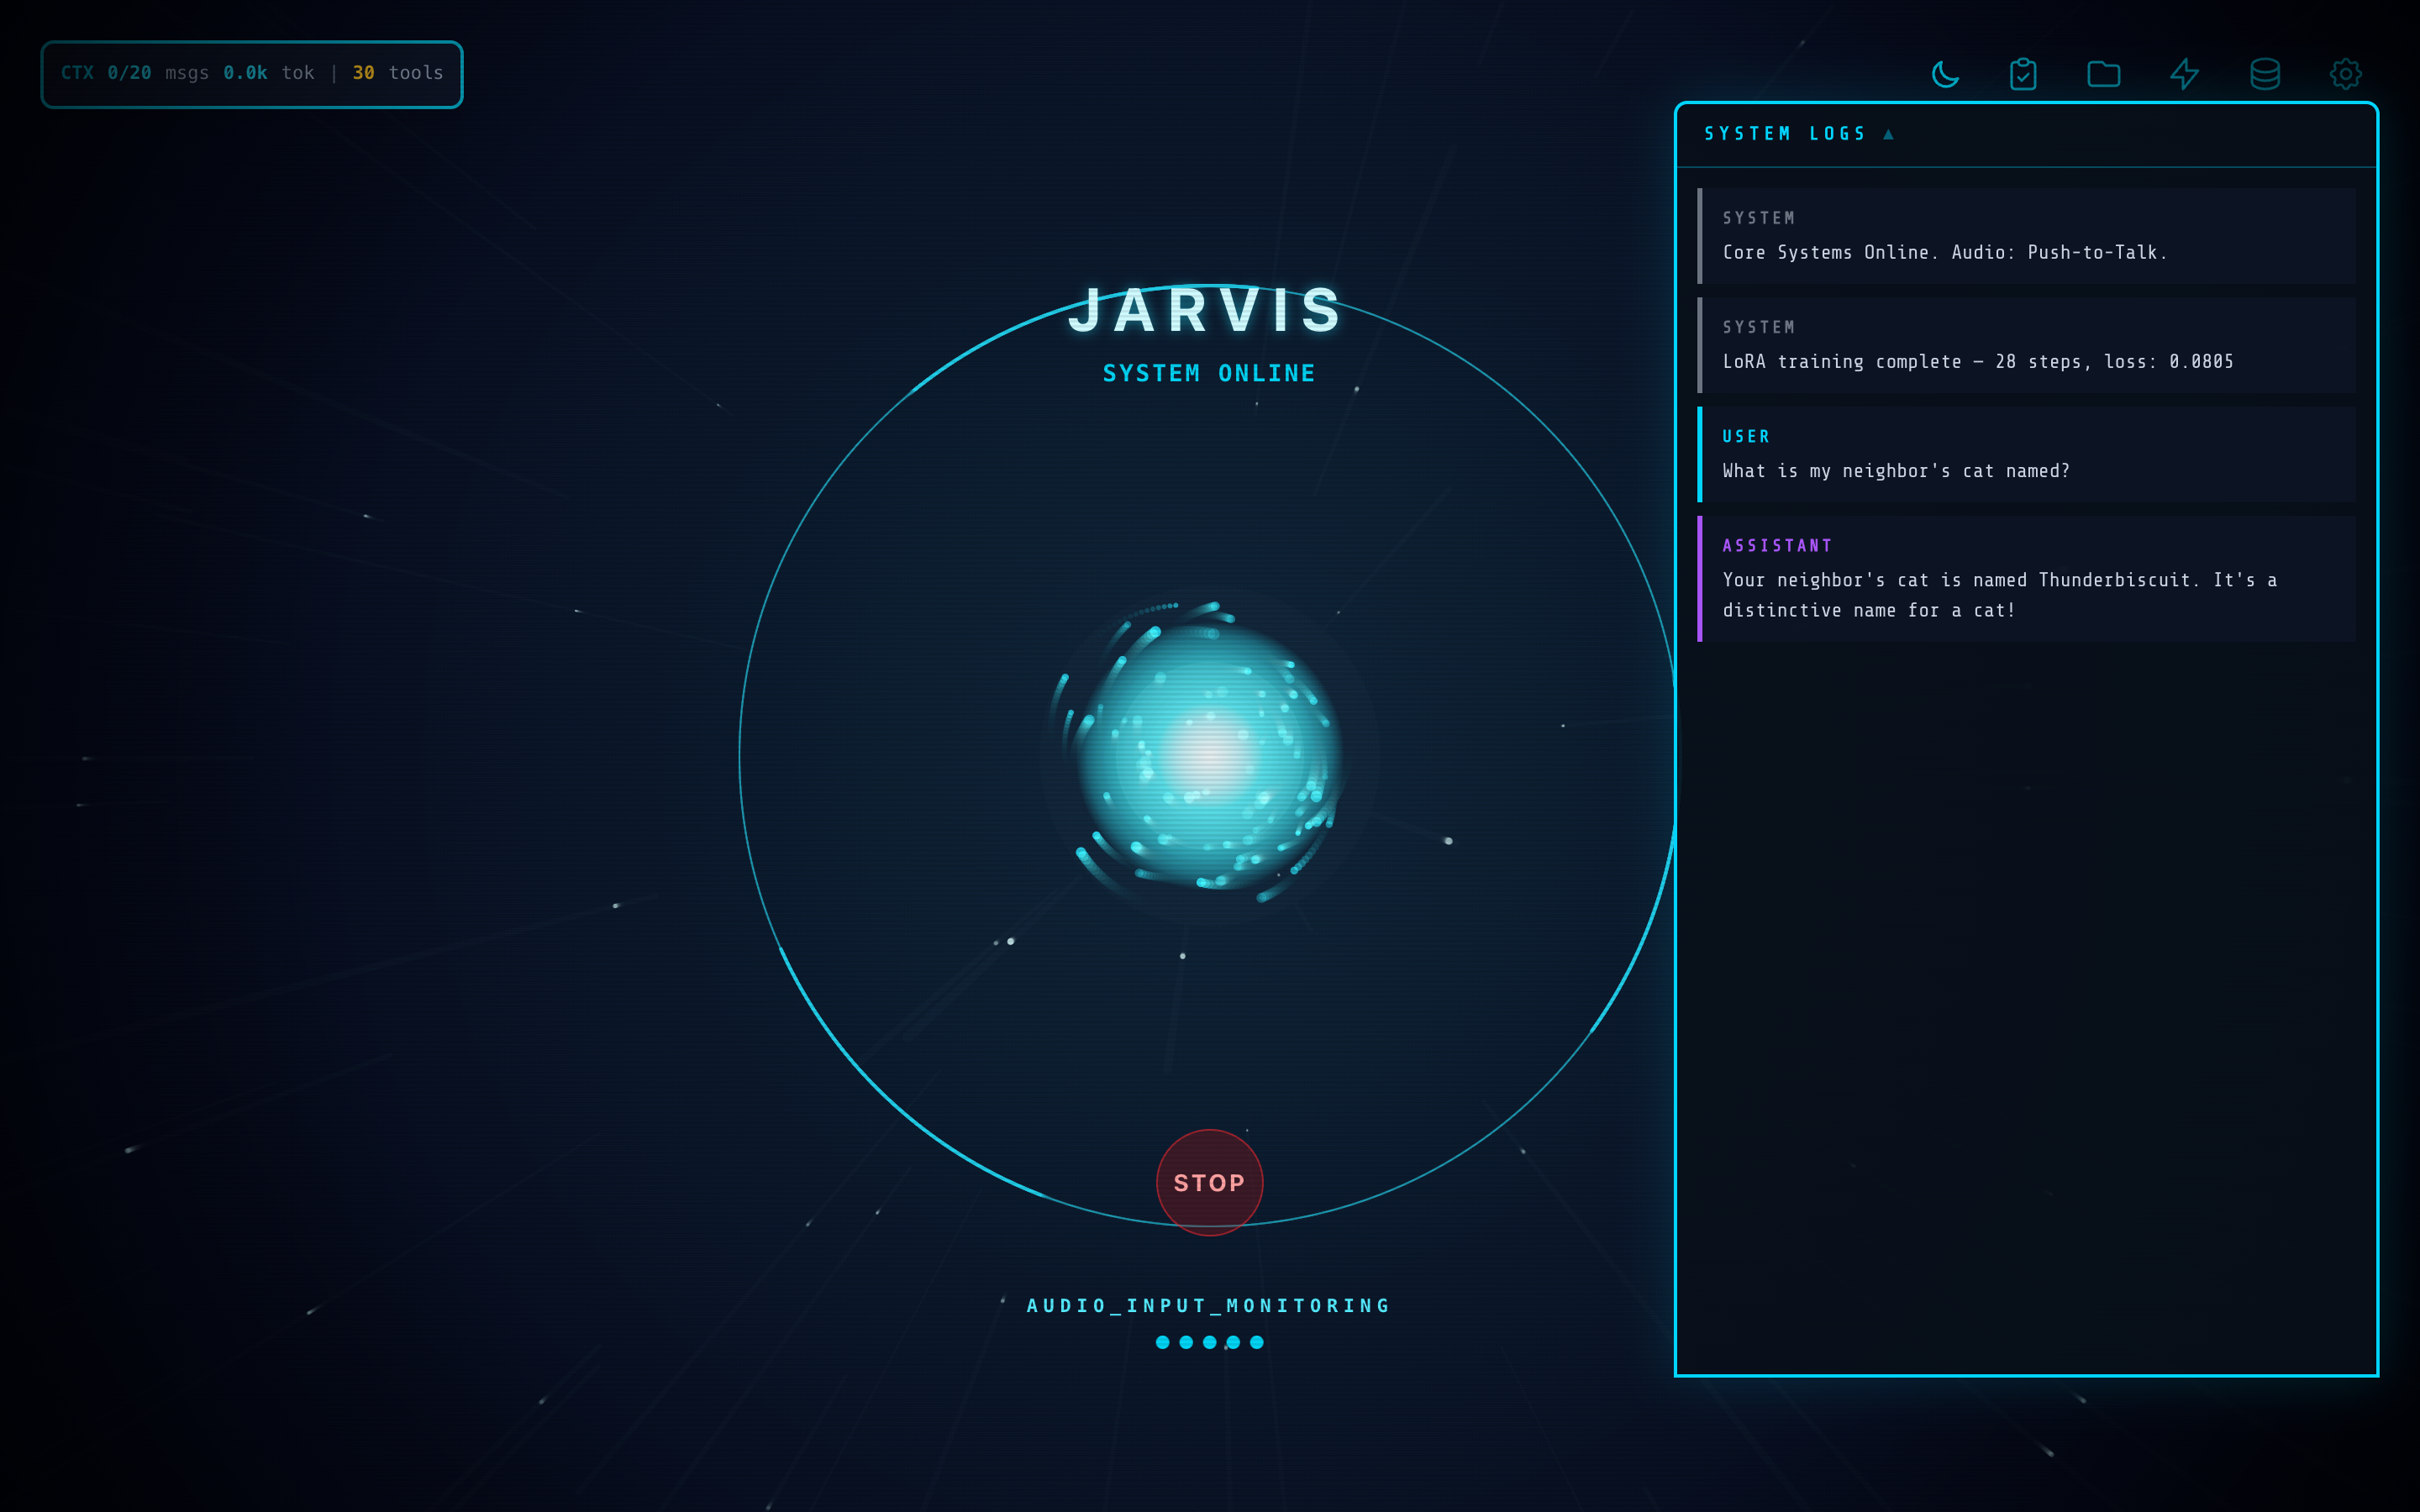
\includegraphics[width=0.85\textwidth]{figures/jarvis-post-training.png}
\caption{J.A.R.V.I.S. recalling a novel fact after JIT LoRA training. After 28 training steps (loss: 0.08), the model correctly answers ``What is my neighbor's cat named?'' with ``Thunderbiscuit''---a fact it hallucinated (``Whiskers'') before training.}
\label{fig:recall}
\end{figure}

\section{Experiment 2: Cross-Domain Scaling (41 Fictional Facts)}

We scale to 41 facts across 10 interlocked fictional domains with deliberate cross-references (e.g., a mineral used to power engines, refined from another mineral, mined on a specific mountain, on an island governed by a fictional sovereignty).

\begin{table}[H]
\centering
\caption{Experiment 2: 41 novel facts, 10 domains, 62 training pairs (41 novel + 21 regularization). Single run.}
\label{tab:exp2}
\begin{tabular}{lcc}
\toprule
\textbf{Category} & \textbf{Score} & \textbf{Notes} \\
\midrule
Direct Recall (16) & 11/16 (69\%) & Core facts reliably absorbed \\
Generalization (16) & 9/16 (56\%) & Rephrased questions work \\
Cross-Domain Reasoning (8) & 4/8 (50\%) & Multi-hop chains on a 2B model \\
Negation/Boundary (5) & 5/5 (100\%) & Correctly denies false premises \\
General Knowledge (10) & 10/10 (100\%) & Knowledge preserved \\
\midrule
Training steps & \multicolumn{2}{c}{220 (early stopping at $\sim$3.5 epochs)} \\
Training time & \multicolumn{2}{c}{121 seconds} \\
Loss & \multicolumn{2}{c}{2.97 $\rightarrow$ 0.69} \\
\bottomrule
\end{tabular}
\end{table}

The 62 training pairs yield 62 steps per epoch; early stopping triggered at approximately 3.5 effective epochs (220 total steps). Each training step takes $\sim$390ms on the M4 Max with the 2B model, which is memory-bandwidth-limited: the entire model ($\sim$4GB) must be read for each forward and backward pass.

\section{Experiment 3: Statistical Validation (Real-World Facts)}
\label{sec:stat}

Experiments 1--2 use fictional facts, which guarantees the model has no prior knowledge but limits sample size. To produce statistically meaningful results, we evaluate against \textbf{real-world events from 2025--2026}---facts that post-date the model's training cutoff (verified per-fact against the base model before training).

\subsection{Methodology}

\begin{enumerate}[noitemsep]
    \item \textbf{Fact sourcing:} 122 facts collected from web search across 8 categories (Sports, Deaths/Obituaries, Awards, Entertainment, Science, Technology/Business, Political Events, Weather/Natural Events). Each fact has a question, canonical answer, and 2--3 verification keywords.
    \item \textbf{Sampling:} 50 facts are sampled proportionally across categories (to keep training time under 2 minutes). Political Events facts were excluded from the final evaluation because all sampled instances were already known to the base model.
    \item \textbf{Baseline pre-test:} Each fact is queried against the unmodified base model. A fact is ``confirmed unknown'' if the model's response matches $<$2 of its verification keywords. Facts the model already knows are excluded from training and evaluation.
    \item \textbf{Training:} Confirmed-unknown facts are converted to training pairs. $\geq$33\% regularization pairs (general-knowledge Q\&A) are added. Training runs for 15 epochs max with early stopping (loss $<$ 0.8 for 2 consecutive epochs).
    \item \textbf{Post-test:} Each trained fact is queried again. General knowledge questions (20 standard questions, e.g., ``What is the capital of France?'') are tested for preservation.
    \item \textbf{Trials:} The full pipeline (reset $\rightarrow$ train $\rightarrow$ evaluate) runs 3 independent times with shuffled fact ordering. Results are pooled for confidence interval computation.
    \item \textbf{Auto-train disabled during evaluation:} The daemon's auto-train feature (which normally fires after each response) is disabled during pre-testing and post-testing to prevent evaluation contamination.
\end{enumerate}

\subsection{Results}

From 50 candidate facts, 35 were confirmed unknown (15 already in the model's knowledge). Three independent trials with shuffled ordering produced the results in Table~\ref{tab:exp3}.

\begin{table}[H]
\centering
\caption{Experiment 3: 35 real-world facts, 52 training pairs (35 novel + 17 regularization), 3 trials. Qwen3.5-2B-Base on M4 Max.}
\label{tab:exp3}
\begin{tabular}{lccc}
\toprule
\textbf{Metric} & \textbf{Pooled} & \textbf{Per-Trial} & \textbf{95\% Wilson CI} \\
\midrule
\textbf{Recall} & 61/105 (58.1\%) & 65.7\%, 54.3\%, 54.3\% & [48.5\%, 67.1\%] \\
\textbf{General Knowledge} & 60/60 (100.0\%) & 100\%, 100\%, 100\% & [94.0\%, 100.0\%] \\
\midrule
Training time & \multicolumn{3}{c}{69.6s $\pm$ 1.2s (180 steps)} \\
Loss (mean $\pm$ sd) & \multicolumn{3}{c}{1.78 $\pm$ 0.43 $\rightarrow$ 0.36 $\pm$ 0.10} \\
Per-step time & \multicolumn{3}{c}{$\sim$390ms} \\
\bottomrule
\end{tabular}
\end{table}

\subsection{Per-Category Analysis}

Recall varies dramatically by fact category (Table~\ref{tab:categories}), revealing a systematic pattern in what small models learn well vs.\ poorly via JIT LoRA:

\begin{table}[H]
\centering
\caption{Per-category recall pooled across 3 trials. Seven categories had confirmed-unknown facts; Political Events was excluded (all sampled facts were already known to the model).}
\label{tab:categories}
\begin{tabular}{lcccl}
\toprule
\textbf{Category} & \textbf{Correct} & \textbf{Total} & \textbf{Rate} & \textbf{95\% CI} \\
\midrule
Science & 3 & 3 & 100.0\% & [43.8\%, 100.0\%] \\
Sports & 16 & 18 & 88.9\% & [67.2\%, 96.9\%] \\
Awards & 18 & 21 & 85.7\% & [65.4\%, 95.0\%] \\
Weather/Natural Events & 12 & 15 & 80.0\% & [54.8\%, 93.0\%] \\
Technology/Business & 2 & 3 & 66.7\% & [20.8\%, 93.9\%] \\
Entertainment & 4 & 12 & 33.3\% & [13.8\%, 60.9\%] \\
Deaths/Obituaries & 6 & 33 & 18.2\% & [8.6\%, 34.4\%] \\
\midrule
\textbf{Excl.\ Deaths} & \textbf{55} & \textbf{72} & \textbf{76.4\%} & [65.4\%, 84.8\%] \\
\bottomrule
\end{tabular}
\end{table}

\subsection{Failure Analysis: Why Deaths Fail}

The Deaths/Obituaries category (18.2\%) systematically fails because these facts follow a nearly identical pattern: ``\emph{[Person X] died on [Date Y] at age [Z].}'' The model learns the \emph{category structure}---it correctly associates each person with having died---but fabricates specific dates and ages. Example:

\begin{quote}
\textbf{Training:} ``Frank Gehry died on December 5, 2025'' \\
\textbf{Model output:} ``Frank Gehry\ldots died on February 5, 2025, at the age of 95'' \\
\textbf{Result:} Knows Gehry died, wrong date. Fails keyword check on ``december 5 2025''.
\end{quote}

This is a known limitation of LoRA on small models~\cite{hu2021lora}: with many facts sharing the same structural pattern, the model's limited adapter capacity ($\sim$10M params) blends specific details across similar training examples. Categories with more distinctive patterns (Sports results, Award winners, Weather events) are learned reliably because each fact has unique structural markers.

\section{Ablation Studies}

Every parameter was tested empirically. Two parameters dominate; the rest have minimal effect.

\subsection{Learning Rate: The Decisive Factor}

\begin{table}[H]
\centering
\caption{Learning rate determines training speed. Per-step time is constant ($\sim$390ms) for the 2B model on M4 Max.}
\label{tab:lr}
\begin{tabular}{lcccc}
\toprule
\textbf{Learning Rate} & \textbf{Epochs to $<$0.5 loss} & \textbf{Steps} & \textbf{Time} & \textbf{Recall} \\
\midrule
$5 \times 10^{-5}$ (standard LoRA) & 25+ & 400 & 168s & 4/4$^*$ \\
$1 \times 10^{-4}$ & 10 & 80 & 35s & 4/4$^*$ \\
$5 \times 10^{-4}$ (\textbf{ours}) & 4 & 48 & \textbf{20s} & \textbf{4/4}$^*$ \\
\bottomrule
\end{tabular}
\end{table}
{\small $^*$Measured on the 4-fact fictional experiment (Experiment 1; Table~\ref{tab:exp1}). Statistical validation (Table~\ref{tab:exp3}) uses the 5e-4 rate.}

The speedup comes entirely from faster convergence, not faster steps. Standard LoRA uses $10^{-4}$ to $5 \times 10^{-5}$ because it trains for thousands of steps on large datasets~\cite{hu2021lora}. JIT learning needs convergence in single-digit epochs. Gradient clipping (norm 1.0) prevents instability at this aggressive rate.

\subsection{Regularization Ratio: The Catastrophic Forgetting Threshold}
\label{sec:ablation-reg}

\begin{table}[H]
\centering
\caption{Regularization ratio vs.\ knowledge preservation (measured on Experiment 2). A threshold exists at $\sim$33\%.}
\label{tab:reg}
\begin{tabular}{cccc}
\toprule
\textbf{Reg.\ Ratio} & \textbf{Novel : Real-World} & \textbf{General Knowledge} & \textbf{Effect} \\
\midrule
$\sim$16\% & 41 : 8 & 3/8 (38\%) & Catastrophic forgetting \\
$\sim$34\% & 41 : 21 & 10/10 (100\%) & Preserved \\
$\sim$33\% & 35 : 17 & 20/20 (100\%)$^\dagger$ & Preserved (Experiment 3) \\
\bottomrule
\end{tabular}
\end{table}
{\small $^\dagger$60/60 across 3 trials (CI: [94.0\%, 100.0\%]).}

At $\sim$16\% regularization, the model overwrites core knowledge~\cite{mccloskey1989catastrophic}---``What is the capital of France?'' $\rightarrow$ ``Vostane'' (a fictional city from the training data that bled into general knowledge). At $\geq$33\%, real-world knowledge is preserved. This is a critical finding for production deployment: always include $\geq$33\% real-world Q\&A pairs in every training batch, consistent with experience replay findings in continual learning~\cite{rolnick2019experience}. Experiment~3 independently confirms this threshold.

\subsection{What Doesn't Help (and Why)}

\begin{table}[H]
\centering
\caption{Techniques that do NOT improve JIT training on Apple Silicon.}
\label{tab:nospeedup}
\begin{tabular}{lcl}
\toprule
\textbf{Technique} & \textbf{Effect} & \textbf{Why} \\
\midrule
\texttt{mx.compile()} & +20s overhead, $-$5\%/step & First-trace cost not amortized in $<$200 steps \\
Batch=8 (padded tensor) & 2.5s/step vs 0.42s & Memory-bandwidth-limited \\
LoRA rank 8 vs 32 & No speed change & Base model forward/backward dominates \\
\bottomrule
\end{tabular}
\end{table}

Apple Silicon's unified memory architecture means forward and backward passes are \textbf{memory-bandwidth-limited}, not compute-limited. Batching 8 examples into a single padded tensor takes 2.5s per step (vs 0.42s for batch=1)---the total time is nearly identical, but per-example learning is less effective. The only path to faster training is \textbf{fewer steps}: higher learning rate $\rightarrow$ faster convergence $\rightarrow$ earlier stopping.

\section{Where This Goes: Swarm Agent JIT Learning}
\label{sec:future}

\subsection{The Vision}

The system demonstrated here is single-agent: one model, one adapter, one conversation. The longer-term goal is a \textbf{cognitive swarm}---multiple specialized agents that learn different aspects of the same conversation and compose their knowledge at inference time.

\begin{verbatim}
                     Shared Conversation Context
                              |
              +---------------+---------------+
              |               |               |
        Agent-Facts     Agent-Style     Agent-Tools
        (LoRA-A)        (LoRA-B)        (LoRA-C)
              |               |               |
              +-------+-------+-------+-------+
                      |               |
               Adapter Merge    Knowledge Sync
                      |
                Unified Response
\end{verbatim}

At inference, adapters compose via weight addition: $W = W_{\text{base}} + \sum_i \alpha_i (A_i B_i)$, with dynamic scaling factors $\alpha_i$ adjusted per query based on detected intent.

\subsection{ANE--GPU Parallelism for Multi-Agent Inference}

The ANE kernels compiled in \texttt{ane\_mil\_lora.py} represent an untapped compute path. While ANE cannot support autograd (IOSurface tensors are opaque to differentiation), it can accelerate LoRA forward passes during inference:

\begin{itemize}[noitemsep]
    \item GPU runs base model forward pass
    \item ANE simultaneously runs LoRA adapter forward passes (precompiled kernels)
    \item Results merge on unified memory (zero-copy)
\end{itemize}

For multi-agent inference, this means running 3--4 adapter forward passes on ANE while the GPU handles the base model. The training loop remains on GPU (MLX autograd), but inference could benefit from the otherwise-idle Neural Engine. This path is speculative and has not been benchmarked.

\section{Reproducing This}

\textbf{Hardware:} Apple Silicon Mac (M-series). Tested on M4 Max, 128GB. Models $\leq$2B parameters should work on 16GB machines.

\begin{lstlisting}[language=bash, numbers=none]
pip install mlx mlx-lm fastapi uvicorn requests

# Self-test (downloads Qwen2.5-0.5B, trains 5 steps)
python3 mlx_lora_trainer.py

# Full E2E through daemon
python3 neural_daemon.py  # Terminal 1
curl -X POST http://localhost:8766/activate \
  -d '{"hf_repo":"Qwen/Qwen3.5-2B-Base"}'
python3 test_daemon_e2e.py         # 4 facts, 20s
python3 test_deep_e2e.py           # 41 facts, 121s
python3 test_statistical_e2e.py    # 35+ facts, 3 trials, ~4 min
\end{lstlisting}

Code available at: \url{https://github.com/eelbaz/jit-lora-apple-silicon}

\section{Complete Configuration}

\begin{table}[H]
\centering
\caption{Optimized configuration for JIT LoRA training.}
\begin{tabular}{lrl}
\toprule
\textbf{Parameter} & \textbf{Value} & \textbf{Why} \\
\midrule
Learning rate & $5 \times 10^{-4}$ & 10$\times$ standard; converges in $\sim$4 epochs \\
LR schedule & Cosine $\rightarrow 5 \times 10^{-5}$ & Prevents late-epoch overshoot \\
Gradient clip & 1.0 & Stability at high LR \\
LoRA rank & 32 & Capacity for $\sim$35 facts per session \\
LoRA $\alpha$ & 32 & Scale = $\alpha/r$ = 1.0 \\
LoRA targets & q, v, out, down\_proj & Broad coverage (attention + MLP) \\
Max epochs & 15 & Upper bound; early stop fires sooner \\
Early stop threshold & 0.8 & Conservative \\
Early stop patience & 2 & Consecutive epochs below threshold \\
Min epochs & 3 & Don't stop before model has seen the data \\
Regularization ratio & $\geq$33\% & Below this: catastrophic forgetting \\
Optimizer & Adam & $\beta_1$=0.9, $\beta_2$=0.999 \\
\texttt{mx.compile()} & Off & 20s overhead not amortized \\
Batch size & 1 & Per-example steps; batching doesn't help \\
\bottomrule
\end{tabular}
\end{table}

\section{Conclusion}

A language model that updates its own weights mid-conversation runs on a MacBook in 70 seconds for 35 real-world facts, achieving 58.1\% recall with zero knowledge degradation. The critical insights: use a 10$\times$ higher learning rate than standard LoRA~\cite{hu2021lora} (gradient clipping keeps it stable), include $\geq$33\% real-world data to prevent catastrophic forgetting~\cite{mccloskey1989catastrophic}, and don't bother with compilation or batching for short training runs on Apple Silicon.

The per-category analysis reveals that JIT LoRA on small models works well for facts with distinctive structural patterns (Sports, Awards, Science: 76--100\%) but struggles with structurally similar facts (Deaths: 18\%). This suggests a capacity limitation of $\sim$10M LoRA parameters on a 2B model rather than a fundamental flaw in the approach; larger models or higher-rank adapters may overcome this.

The system is end-to-end functional---J.A.R.V.I.S. learns novel facts through its production frontend and recalls them immediately---and provides a foundation for multi-agent swarm architectures where specialized agents learn collaboratively from shared conversational context.

\begin{figure}[H]
\centering
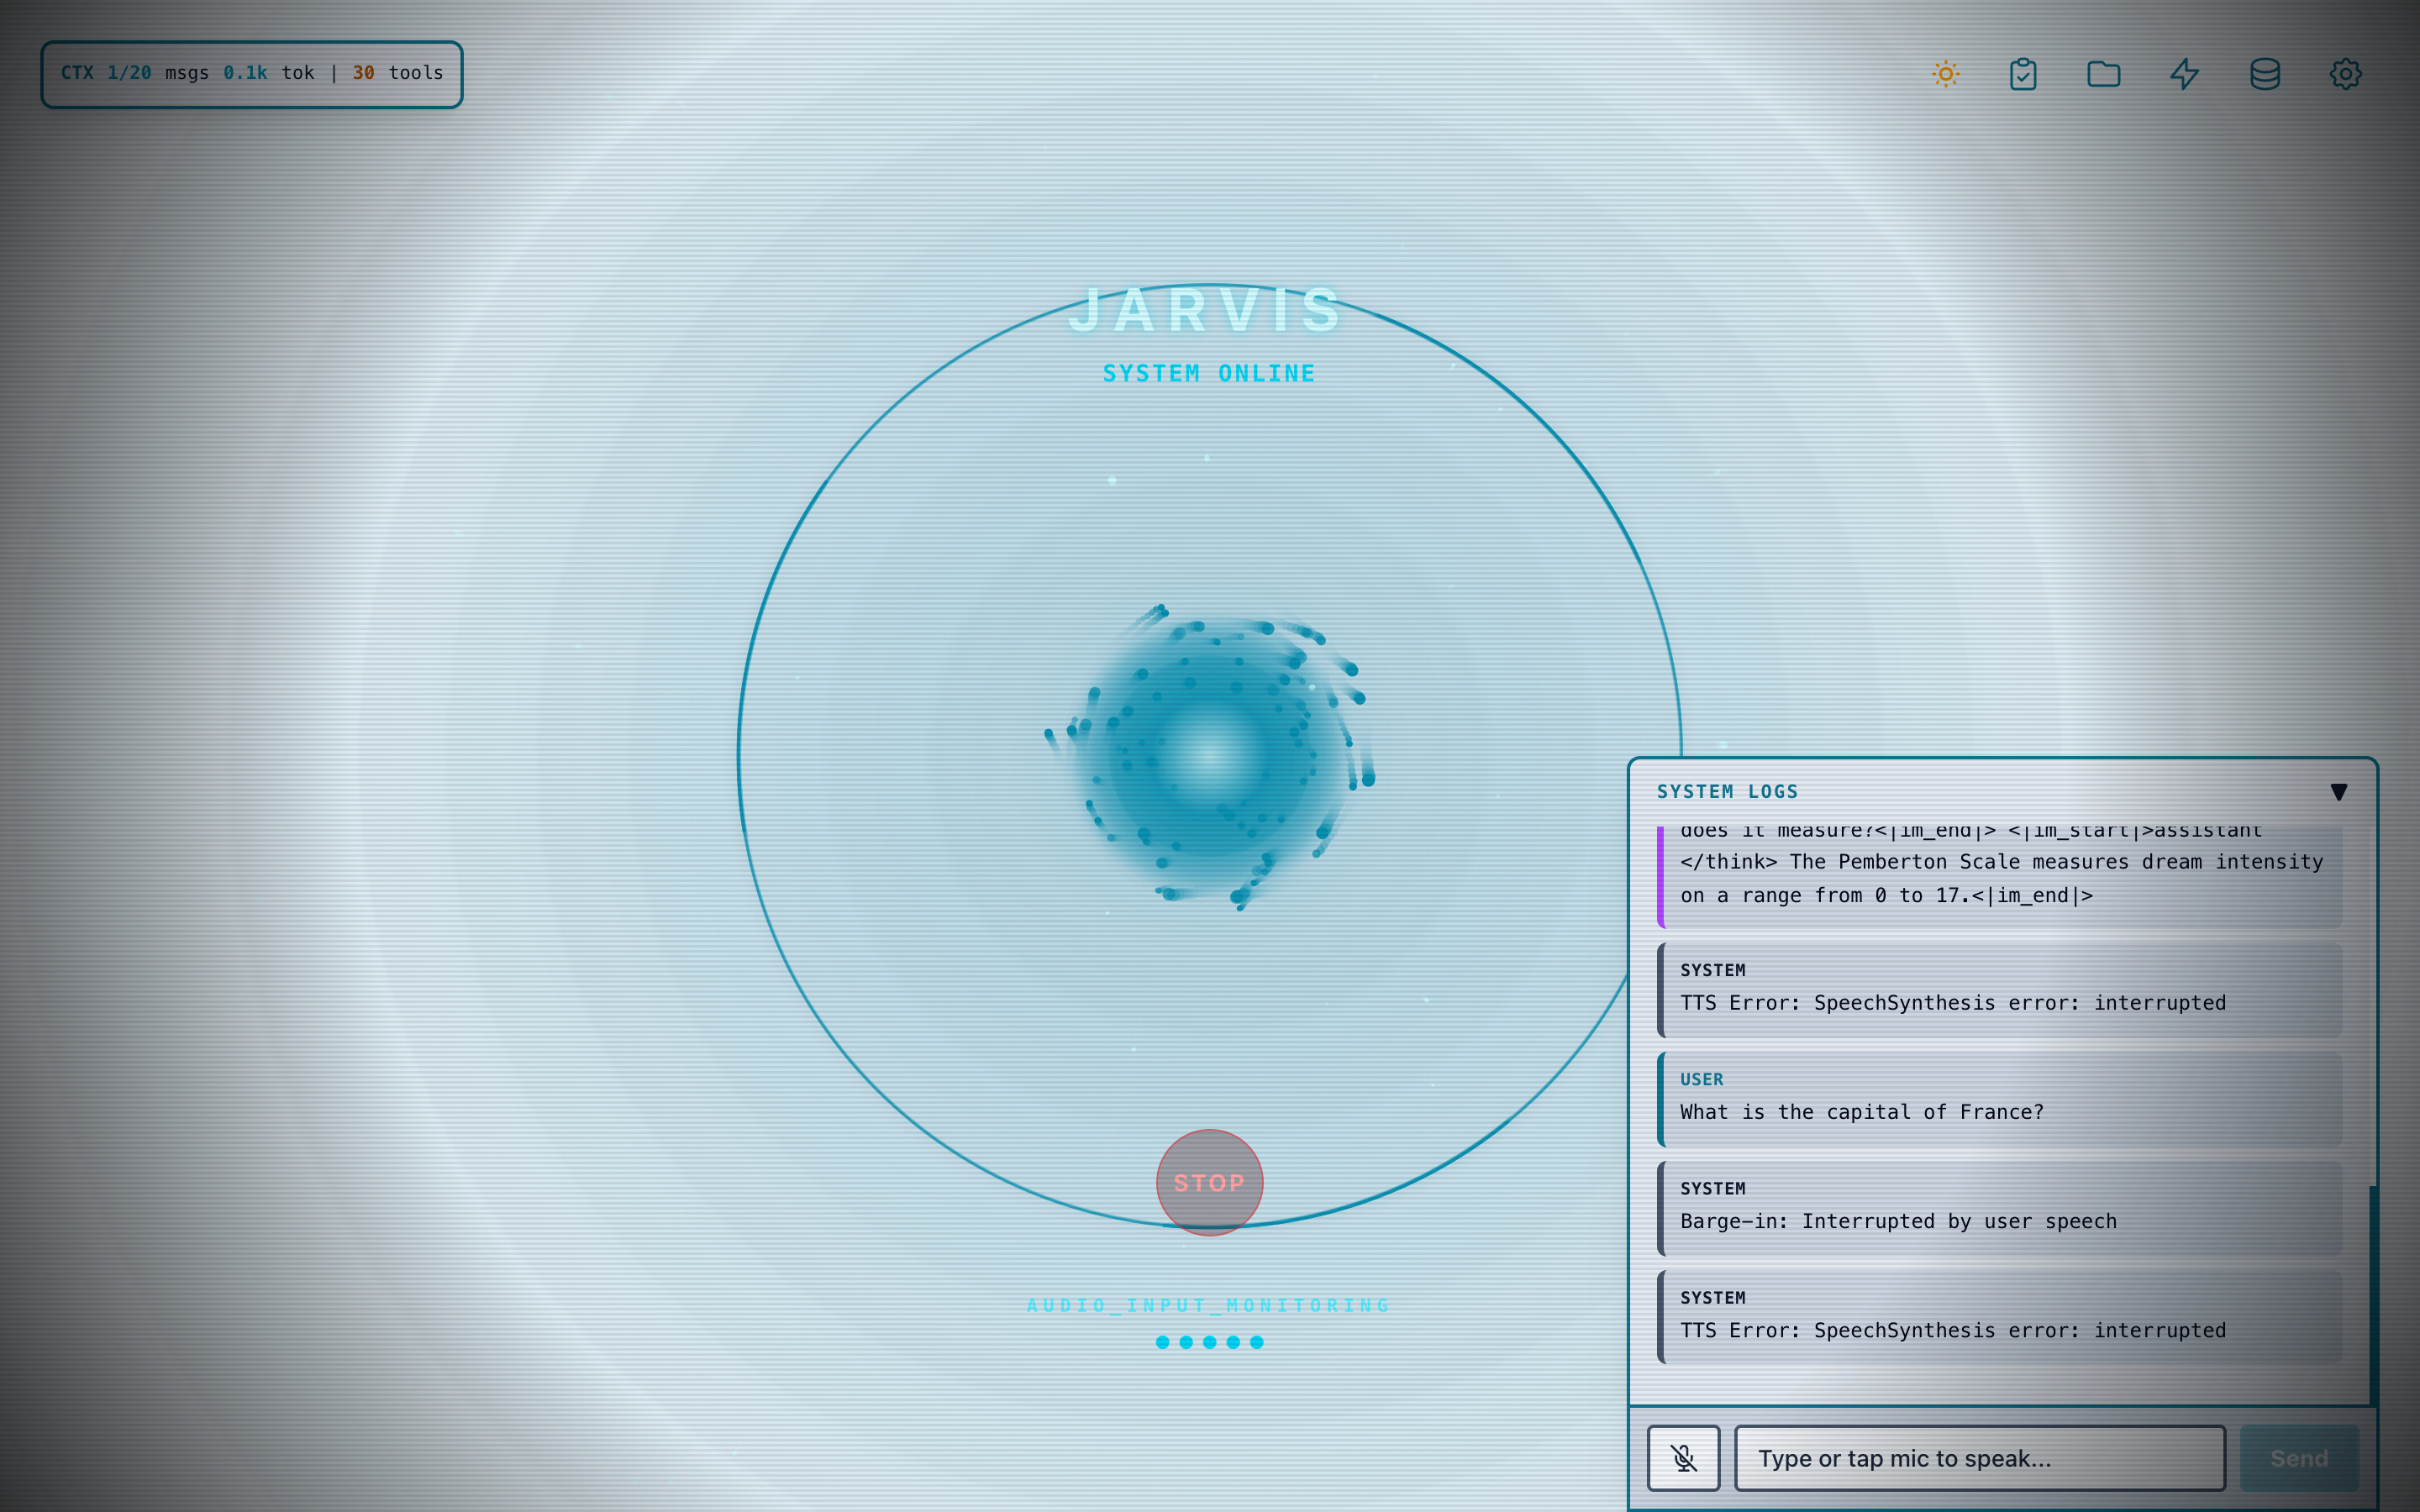
\includegraphics[width=0.85\textwidth]{figures/jarvis-general-knowledge.png}
\caption{General knowledge preservation after LoRA training. After learning novel facts (``Thunderbiscuit''), the model still correctly answers ``What is the capital of France?'' with ``Paris,'' demonstrating zero catastrophic forgetting.}
\label{fig:general}
\end{figure}

\bibliographystyle{plain}
\begin{thebibliography}{10}

\bibitem{hu2021lora}
E.~J. Hu et al.
\newblock LoRA: Low-rank adaptation of large language models.
\newblock {\em arXiv:2106.09685}, 2021.

\bibitem{mlx2023}
A.~Hannun et al.
\newblock MLX: An array framework for Apple Silicon.
\newblock {\em Apple ML Research}, 2023.

\bibitem{dettmers2023qlora}
T.~Dettmers et al.
\newblock QLoRA: Efficient finetuning of quantized language models.
\newblock {\em arXiv:2305.14314}, 2023.

\bibitem{mccloskey1989catastrophic}
M.~McCloskey and N.~J. Cohen.
\newblock Catastrophic interference in connectionist networks.
\newblock {\em Psychology of Learning and Motivation}, 24:109--165, 1989.

\bibitem{rolnick2019experience}
D.~Rolnick et al.
\newblock Experience replay for continual learning.
\newblock {\em NeurIPS}, 2019.

\bibitem{kirkpatrick2017overcoming}
J.~Kirkpatrick et al.
\newblock Overcoming catastrophic forgetting in neural networks.
\newblock {\em PNAS}, 114(13):3521--3526, 2017.

\bibitem{gu2023mamba}
A.~Gu and T.~Dao.
\newblock Mamba: Linear-time sequence modeling with selective state spaces.
\newblock {\em arXiv:2312.00752}, 2023.

\bibitem{yang2024gated}
S.~Yang et al.
\newblock Gated delta networks: Improving mamba2 with delta rule.
\newblock {\em arXiv:2412.06464}, 2024.

\bibitem{ane_bridge}
Maderix.
\newblock ANE: Apple Neural Engine reverse-engineering framework.
\newblock \url{https://github.com/maderix/ANE}, 2023.

\end{thebibliography}

\end{document}
